\documentclass[10pt]{article}

\usepackage[margin=0.65in]{geometry}
\usepackage[T1]{fontenc}
\usepackage[utf8]{inputenc}
\usepackage{lmodern}
\usepackage{microtype}
\usepackage{amsmath}
\usepackage{graphicx}
\usepackage{xcolor}
\usepackage[labelfont=bf]{caption}
\usepackage[round,authoryear]{natbib}
\usepackage{hyperref}
\usepackage{authblk}

\hypersetup{colorlinks=true,linkcolor=blue,citecolor=blue,urlcolor=blue}
\newcommand{\software}[1]{\texttt{#1}}
\newcommand{\placeholder}[1]{\textcolor{red}{\textbf{[#1]}}}

\title{TRIARCHY: a control-aware cross-assay evidence framework for environmental microbiome profiling}
\author[1,2,*]{Alexander G. Lucaci}
\author[3]{Phoebe Ledins}
\author[4]{Elizabeth Henaff}
\author[3]{Anna Dyson}
\author[1,2]{Christopher E. Mason}
\affil[1]{Department of Systems and Computational Biomedicine, Weill Cornell Medicine, New York, NY, USA}
\affil[2]{The HRH Prince Alwaleed Bin Talal Bin Abdulaziz Alsaud Institute for Computational Biomedicine, Weill Cornell Medicine, New York, NY, USA}
\affil[3]{Yale Center for Ecosystems + Architecture, Yale University, New Haven, CT, USA}
\affil[4]{New York University Tandon School of Engineering, New York, NY, USA}
\affil[*]{Correspondence: \href{mailto:agl4001@med.cornell.edu}{agl4001@med.cornell.edu}}
\date{}

\begin{document}
\maketitle

\begin{abstract}
\noindent\textbf{Summary:}
Environmental microbiome studies increasingly combine whole-metagenome shotgun
(WMS), 16S rRNA gene and fungal ITS sequencing, although the assays have
different detection limits, taxonomic resolution and contamination
sensitivities. TRIARCHY is a reproducible workflow and evidence framework that
retains assay-native abundance estimates while harmonizing taxonomy and
experimentally linked controls. For each sample--taxon pair, it estimates a
cross-assay authenticity score and assigns an interpretable explanation for
agreement or discordance. In 1,562 synthetic truth-labelled observations,
TRIARCHY achieved the highest explanatory-status accuracy (0.811) and lowest
Brier score (0.371) among the evaluated integration strategies.

\smallskip\noindent\textbf{Availability and Implementation:}
TRIARCHY is implemented in Nextflow DSL2 and Python, supports Docker and
Apptainer, and is available under GPL-3.0-only at
\url{https://github.com/aglucaci/TRIARCHY}. Versioned source and benchmark
archives will be available at \placeholder{release DOI}.

\smallskip\noindent\textbf{Contact:}
\href{mailto:agl4001@med.cornell.edu}{agl4001@med.cornell.edu}

\smallskip\noindent\textbf{Supplementary information:}
Supplementary data are available at \emph{Bioinformatics} online.
\end{abstract}

\section{Introduction}

Environmental microbiome studies increasingly profile the same samples using
WMS, 16S and ITS sequencing. These assays provide complementary observations,
not interchangeable measurements. Primer amplification and marker copy number
shape amplicon profiles, whereas sequencing depth, host fraction and genome
size affect shotgun detection. Biomass, contamination, reference-database
coverage and taxonomic resolution influence all three. Consequently, absence
from one assay does not imply biological absence, and disagreement does not
necessarily represent biological discordance.

Existing tools solve important parts of this problem. Common-reference systems
can improve taxonomic compatibility across data types \citep{mcdonald2024};
\software{decontam} identifies contaminants within marker-gene and metagenomic
studies \citep{davis2018}; and Qmatey and Com-2seq support cross-platform
profiling or statistical integration \citep{adams2023,yue2025}. These
approaches primarily harmonize taxonomy, remove contaminants or combine
abundance profiles. They do not jointly interpret matched WMS--16S--ITS
observations using experimentally linked controls, assay detectability,
taxonomic compatibility and reference representation.
Incomplete and uneven fungal reference resources are a particular limitation
for shotgun mycobiome interpretation \citep{avershina2025}.

TRIARCHY addresses evidence adjudication rather than abundance pooling. For
each sample--taxon pair, it first evaluates whether the available observations
support biological authenticity and then determines whether cross-assay
agreement or disagreement is best explained by concordance, assay limitation,
taxonomic limitation, contamination, genuine discordance or insufficient
evidence. Assay-native outputs and provenance remain available for inspection.
Here, we describe the workflow and evaluate its evidence logic using
truth-labelled synthetic benchmarks and a matched 51-library showcase.

\section{Implementation}

\subsection{Workflow architecture}

TRIARCHY is a Nextflow DSL2 workflow \citep{ditommaso2017} that accepts a
sample table, sequencing manifest, paired-control table and evidence policy
(Fig.~\ref{fig:triarchy-main}). Its assay-native branches process WMS reads
with \software{fastp}, Bowtie2, Kraken~2, Bracken and HUMAnN
\citep{chen2018,langmead2012,wood2019,lu2017,beghini2021}; 16S reads with
Cutadapt, DADA2 and SILVA
\citep{martin2011,callahan2016,quast2013}; and ITS reads with Cutadapt, ITSxpress, DADA2
and a configured fungal reference \citep{martin2011,rivers2018,einarsson2024}.
These branches provide supporting infrastructure; the methodological
contribution is the control-aware integration layer. Inputs undergo metadata,
paired-read and database preflight checks before expensive tasks are scheduled.

\subsection{Experimentally linked controls}

TRIARCHY represents the experiment as a graph $G=(S,C,E)$, where $S$ is
the set of biological samples, $C$ is the set of controls and $E$ contains
valid experimental relationships. Field, extraction, PCR, library and
sequencing controls are linked only to the samples, assays and batches for
which they are informative. The workflow rejects cross-assay edges, cycles,
unknown identifiers and incompatible batches. For every taxon, linked-control
prevalence, control-to-sample abundance enrichment and batch localization are
combined into stage-specific contamination evidence. This design avoids
treating every blank as a global negative control and preserves the laboratory
stage responsible for a warning.

\subsection{Taxonomic harmonization}

Source assignments are mapped to canonical taxa while retaining the original
database, identifier, lineage, mapping method, mapping confidence and reference
coverage. Comparisons are made at the deepest mutually defensible rank. Thus,
a WMS assignment to \emph{Escherichia coli} and a 16S assignment to
\emph{Escherichia} constitute genus-level, rank-limited agreement rather than
species-level conflict. Original assay-native tables are never overwritten or
averaged.

\subsection{Two-stage evidence model}

All terms are evaluated separately for biological sample $s$, canonical taxon
$t$ and assay $m\in\{\mathrm{WMS},\mathrm{16S},\mathrm{ITS}\}$; $j$ indexes
the control stage (field, extraction, PCR, library, sequencing run or other).
Except for depths, ranks, indicators and log odds, component scores are bounded
to $[0,1]$. Linked-control evidence is summarized as
\begin{equation}
 C_{smt}=\min\{1,\;0.45A_{smt}+0.35P_{smt}+0.20B_{smt}\},
 \label{eq:contamination}
\end{equation}
where $C_{smt}$ is the overall control-derived contamination score,
$A_{smt}$ is the largest abundance ratio between a linked control and its
biological sample, $P_{smt}$ is taxon prevalence in linked controls scaled by
prevalence in biological samples, and $B_{smt}$ is batch-localization evidence.
The weights 0.45, 0.35 and 0.20 represent abundance enrichment, prevalence and
batch localization, respectively; the minimum operation caps the score at one.
Detection power for an expected, measured assay is
\begin{equation}
 \pi_{smt}=R_{mt}\left(1-\exp\{-d_{sm}/D_m\}\right)G_{mt}Q_{sm},
 \label{eq:detection-power}
\end{equation}
Here, $\pi_{smt}$ is the estimated ability of assay $m$ to detect taxon $t$ in
sample $s$ if present; $R_{mt}$ is the configured assay reliability for the
taxon's kingdom; $d_{sm}$ is observed library depth; and $D_m$ is the
assay-specific depth scale at which the saturation curve begins to level.
$G_{mt}$ is database or reference coverage, and $Q_{sm}$ is a QC factor: one
for a passing library, zero for an unusable library and a reduced value for a
low-depth, host-dominated or review-status library. An unmeasured assay receives
zero detection power and supplies no negative evidence. Positive per-assay
evidence is
\begin{equation}
 e_{smt}=\left(1-\exp\{-5x_{smt}\}\right)\sqrt{1/r_{smt}}\,
 \lambda_{smt}\mu_{smt}R_{mt}\kappa_{smt}(1-C_{smt}),
 \label{eq:assay-evidence}
\end{equation}
Here, $e_{smt}$ is positive evidence supplied by a detection; $x_{smt}$ is
assay-native normalized abundance; and $1-\exp(-5x_{smt})$ is a saturating term
that prevents high-abundance calls from dominating. $r_{smt}\geq1$ is
within-library abundance rank, so the square-root term favors higher-ranked
detections. $\lambda_{smt}$ is canonical taxonomic-rank resolution scaled from
zero (unclassified) to one (species), $\mu_{smt}$ is mapping confidence,
$R_{mt}$ is assay reliability, $\kappa_{smt}$ is primer compatibility, and
$1-C_{smt}$ discounts detections also supported by controls.

Stage I updates prior log odds using positive detections, technically adequate
nondetections and contamination penalties:
\begin{equation}
\begin{split}
 \ell_{st}=\ell_0+\sum_{m\in M_t}\Bigg[
 I^+_{smt}\left(4e_{smt}+\log\frac{\pi_{smt}+0.05}{f_{smt}+0.05}\right)\\
 {}+I^-_{smt}\log\frac{1-\pi_{smt}}{1-f_{smt}}\Bigg]
 -3\max_m C_{smt}-2\max_j S_{stj},
\end{split}
\label{eq:log-odds}
\end{equation}
Here, $\ell_{st}$ is updated authenticity log odds and
$\ell_0=\log[p_0/(1-p_0)]$ is prior log odds for configured presence prior
$p_0$ (default 0.25). $M_t$ is the kingdom-appropriate assay set: WMS and 16S
for bacterial or archaeal taxa, and WMS and ITS for fungi. $I^+_{smt}=1$ when
an expected assay detects the taxon; $I^-_{smt}=1$ when it was measured but did
not detect the taxon. Both are zero otherwise. $f_{smt}$ is the baseline
false-positive rate after contamination adjustment, and $S_{stj}$ is the
contamination score at control stage $j$. The 0.05 constants stabilize ratios
near zero; 4, 3 and 2 weight positive evidence, maximum assay contamination and
maximum stage-specific contamination. The authenticity score is
\begin{equation}
 \theta_{st}=\frac{1}{1+\exp\{-\ell_{st}\}},
 \label{eq:authenticity}
\end{equation}
which maps log odds $\ell_{st}$ through the logistic function to the reported
score $\theta_{st}$. Its approximate interval is
\begin{equation}
 \theta_{st}\;\mathbin{\pm}\;
 1.96\sqrt{\frac{\theta_{st}(1-\theta_{st})}{\max(2,\;2+n_{st})}},
 \label{eq:authenticity-interval}
\end{equation}
where $n_{st}$ is the sum over expected assays of measurement and detection
indicators plus detection power, mapping confidence and reference coverage. It
is an effective evidence count, not a sample size. The factor 1.96 gives an
approximate 95\% interval, the denominator is floored at two, and reported
limits are truncated to $[0,1]$. Because the interval is heuristic and the
model is calibrated only on synthetic data, $\theta_{st}$ is termed an
authenticity score rather than a probability of biological presence.

Stage II assigns one of six parent explanations: \emph{concordant},
\emph{assay-limited}, \emph{taxonomy-limited},
\emph{contamination-associated}, \emph{genuine discordance} or
\emph{indeterminate}. Detailed statuses distinguish, for example,
single-assay credible detections, reference limitations and cross-contamination
candidates. Every row reports the status, score interval, decision reason,
assay evidence, control evidence and provenance. Missing-by-design assays
reduce the scope of inference rather than being interpreted as nondetections.
The rules are evaluated in a fixed order. A taxon first becomes
\emph{contamination-associated} if its maximum $C_{smt}$ exceeds the configured
contaminant threshold, or if both contamination and batch-localization scores
exceed their cross-contamination thresholds. Explicitly incompatible canonical
assignments produce \emph{genuine discordance}. Detection by every assay in
$M_t$ is \emph{concordant}, unless agreement requires roll-up to different
taxonomic ranks, in which case it is \emph{taxonomy-limited}. With one positive
assay, an unmeasured partner is treated as credible single-assay evidence; low
$G_{mt}$ gives a reference-limited classification, low $\pi_{smt}$ gives an
assay-limited nondetection, and high $\pi_{smt}$ with no detection gives genuine
discordance. Intermediate or absent usable evidence is \emph{indeterminate}.
The separate authenticity state is \emph{biologically supported} only when the
score and its lower interval limit exceed configured support thresholds,
\emph{not supported} only when the score and upper limit fall below absence
thresholds, and \emph{indeterminate} otherwise. Thus Stage I estimates strength
of biological support, whereas Stage II explains the observed cross-assay
pattern. Exact thresholds are supplied in the versioned evidence-policy file.

\section{Results}

\subsection{Frozen synthetic truth suite}

The frozen synthetic truth suite comprises repository-generated challenge
fixtures. Each fixture encodes synthetic taxon truth,
sample--control edges, read origins, taxonomic crosswalks and expected evidence
statuses. These datasets are important because every expected detection,
contaminant and explanation is known exactly, permitting deterministic
regression testing that is impossible in an observational cohort. Together
they test metadata validation, rank-aware harmonization, stage-specific
contamination, assay-limited nondetection and explanatory classification. We
compared independent assay interpretation, naive genus-table concatenation,
shared-taxonomy harmonization, per-assay contamination filtering, global
negative-control filtering and TRIARCHY against the same truth tables.

For truth-labelled observations, authentic-taxon and contaminant performance
use
\begin{equation}
 \mathrm{precision}=\frac{\mathrm{TP}}{\mathrm{TP}+\mathrm{FP}},\qquad
 \mathrm{recall}=\frac{\mathrm{TP}}{\mathrm{TP}+\mathrm{FN}},\qquad
 F_1=\frac{2\,\mathrm{precision}\,\mathrm{recall}}
 {\mathrm{precision}+\mathrm{recall}},
 \label{eq:f1}
\end{equation}
and score calibration is summarized by the Brier score \citep{brier1950},
\begin{equation}
 \mathrm{Brier}=\frac{1}{N}\sum_{i=1}^{N}(\theta_i-y_i)^2,
 \label{eq:brier}
\end{equation}
where $y_i$ is the truth label and $\theta_i$ is the reported authenticity
score.

Replaying the integration and comparison pipeline on the committed synthetic
profiles yielded 1,562 collapsed
sample--taxon truth observations. TRIARCHY achieved explanatory-status accuracy
of 0.811, compared with 0.774 for per-assay contamination filtering, 0.758 for
naive concatenation and 0.665 for shared taxonomy. It also had the lowest Brier
score (0.371 versus 0.488--0.626 for the evaluated alternatives) and matched
per-assay contamination filtering for contaminant $F_1$ (0.660). Its false
concordance rate was 0.058, compared with 0.242 for naive concatenation.

The strict released \software{biological\_state=present} endpoint produced no
positive calls and therefore an authentic-taxon $F_1$ of 0.000. This result
reflects a conservative policy: evidence can support an explanatory status
while the authenticity interval still overlaps a decision threshold. We
report this limitation explicitly because the score is not yet calibrated on
an external physical benchmark. By contrast, per-assay contamination filtering
achieved authentic-taxon $F_1=0.936$ in the same synthetic comparison.
TRIARCHY's present advantage is therefore explanatory classification and
auditable evidence reporting, not superior authentic-taxon recovery.

\subsection{Matched WMS--16S--ITS synthetic showcase}

The matched-assay synthetic showcase is a repository-generated, 19-sample and
51-library WMS--16S--ITS dataset. It includes biological samples, extraction and PCR
blanks, WMS library blanks and a positive mixed-community control. Designed
signals cover host DNA, reagent and batch contamination, primer bias,
taxonomic ambiguity, fungal reference limitation and pathway reporting. The
dataset is important because it exercises the complete workflow graph and
reporting contract in a single reproducible run. It tests task orchestration,
control linkage, all three assay branches, integration and output provenance;
its scaled reads are not independent empirical biological evidence.

The matched-assay showcase completed 163 Nextflow tasks with no failed tasks and emitted 60
sample--taxon evidence rows while preserving assay-specific outputs. In the
lightweight resource profile, a compact five-dataset bundle containing 97
modality-specific libraries completed in 60.18~s with a peak observed
process-tree resident set size of 0.372~GiB. These measurements characterize
workflow orchestration with scaled inputs, not production database
classification. Docker and Apptainer hooks and workstation, Slurm and cloud
configuration templates are included; production runtime and external
physical/environmental validation remain required before a final performance
claim.

\subsection{Six-protocol extraction comparison cohort}

The six-protocol extraction comparison cohort comes from the UC San Diego
study by Shaffer \emph{et al.} (ENA ERP124610; BioProject PRJEB40903; Qiita
12201) \citep{shaffer2022extraction}. The study contains bacterial and fungal
community material profiled by WMS, 16S and ITS, together with blanks and
experimental dilution structure. It is the most important external dataset for
TRIARCHY because physical material and laboratory controls provide a test of
whether the evidence model can distinguish authentic low-abundance organisms
from extraction-associated contamination and assay-specific nondetection.

The current curated subset contains three matched biological groups, each with
WMS, 16S and ITS data. Across those triplets and the available blanks, the
subset contains 11 ENA runs represented by 15 FASTQ files: four WMS, four 16S
and three ITS runs, comprising nine biological libraries and two negative
controls. All 2.96~MB of selected data passed ENA MD5 and gzip validation. No
cross-assay control edges could be recovered reliably from the public metadata,
so the generated control relationship table remains empty. Consequently,
matched-assay download and integrity validation are complete, but control-aware
biological performance has not yet been estimated; contamination results must
not be interpreted until those relationships are manually curated.

\section{Conclusion}

TRIARCHY is an evidence-interpretation layer for microbiome studies that use
matched WMS, 16S, ITS and controls. It is neither a new read classifier nor an
abundance-merging algorithm. Instead, it preserves assay-native measurements
while distinguishing robust agreement from assay limitation, taxonomic
ambiguity, reference incompleteness and experimental contamination. The
current deterministic benchmarks support the implementation and explanatory
logic but also identify a conservative authenticity threshold that requires
external calibration. Future releases will calibrate the score across physical
mock communities and environmental cohorts and extend the evidence model to
additional assays.

\begin{figure}[t]
  \centering
  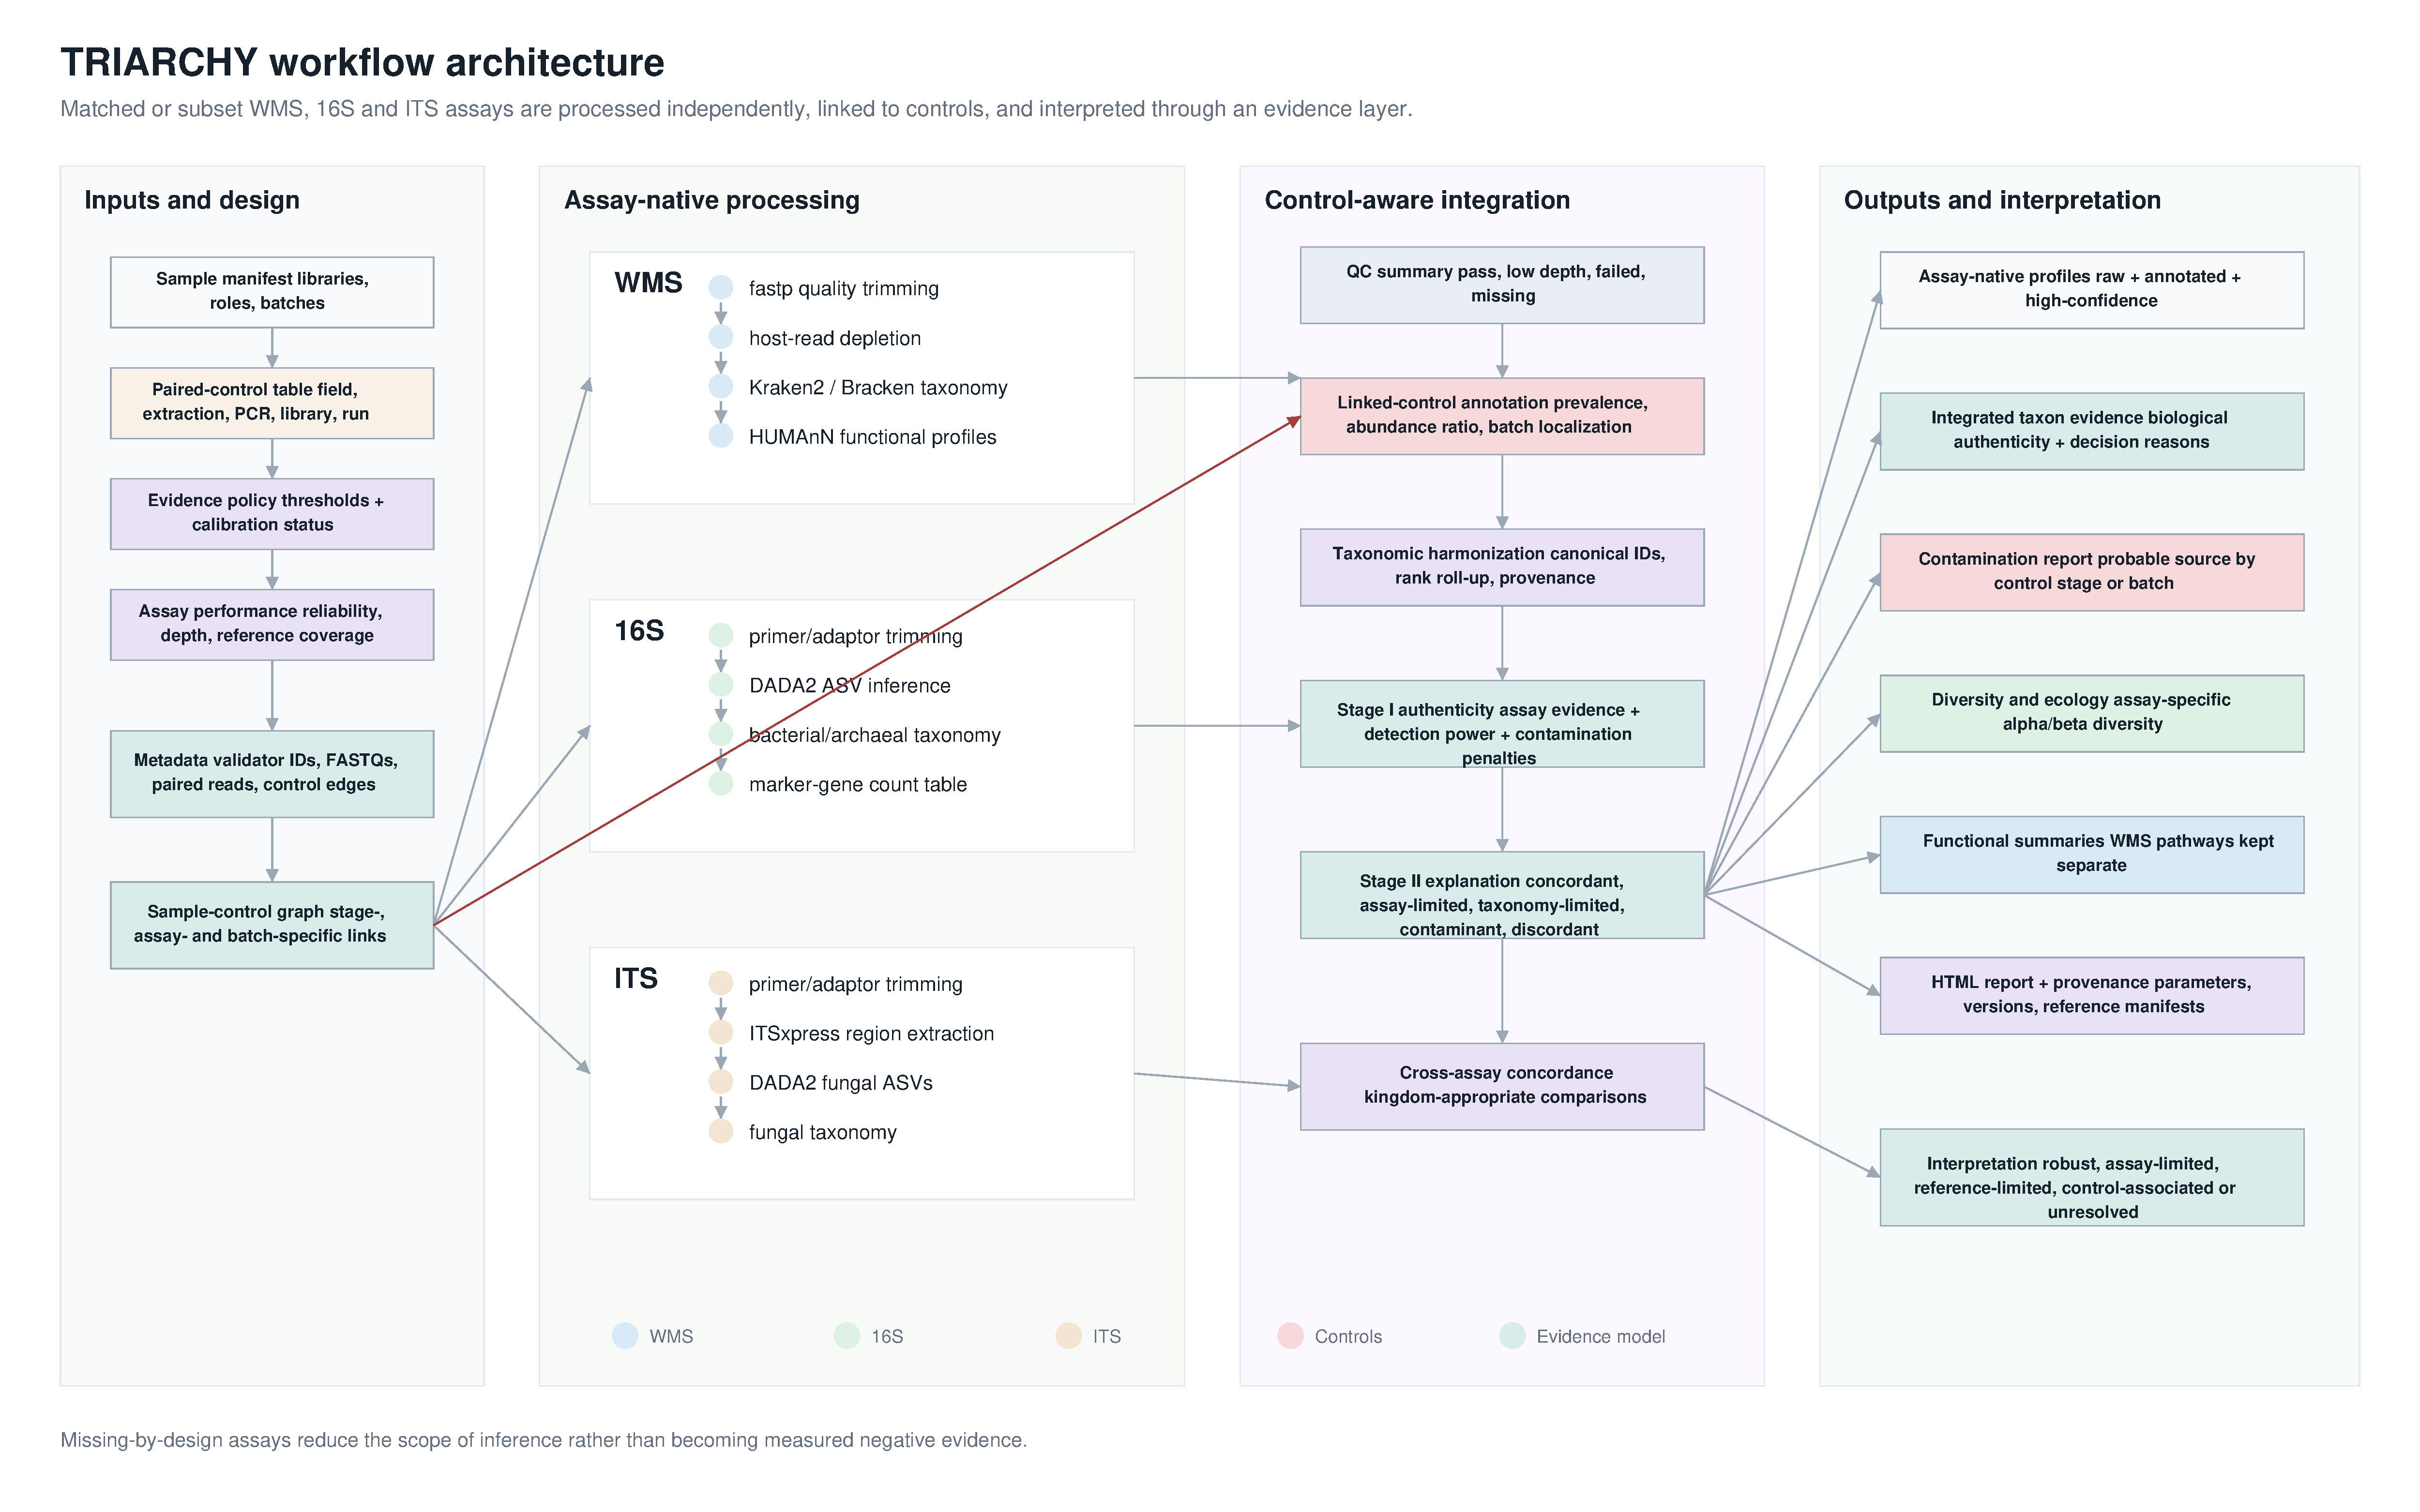
\includegraphics[width=\linewidth]{figures/figure1_workflow_architecture.pdf}
  \caption{\textbf{TRIARCHY architecture and evidence flow.} (A) Biological samples and
  experimentally relevant controls form a stage-, assay- and batch-specific
  graph. (B) WMS, 16S and ITS libraries retain their assay-native processing
  and abundance measurements. (C) Taxonomic harmonization feeds a two-stage
  model that first scores biological authenticity and then explains the
  cross-assay pattern using detection, quality, mapping, reference and control
  evidence. (D) Each sample--taxon pair receives an interpretable status and
  auditable decision reason.}
  \label{fig:triarchy-main}
\end{figure}

\section*{Data availability}
Source code, deterministic test data, benchmark truth tables and reference
manifests are available at \url{https://github.com/aglucaci/TRIARCHY}.
The frozen submission release will be archived at \placeholder{release DOI}.

\section*{Acknowledgements}
The authors thank the members of the Mason Lab for workflow design, benchmark
generation and environmental sampling input.

\section*{Funding}
This work was supported by \placeholder{funding agency and grant number}.

\section*{Conflict of interest}
The authors declare no competing interests.

\bibliographystyle{plainnat}
\bibliography{references}

\end{document}
